\begin{flushleft}
    Wie in unserer Evaluation der Lösungsideen bereits beschrieben übernimmt der ESP32 Microcontroller, siehe Abbildung \ref{fig:esp32_mc}, die Steuerung unseres Roboters. 
    
    \begin{figure}[h!]
        \centering
        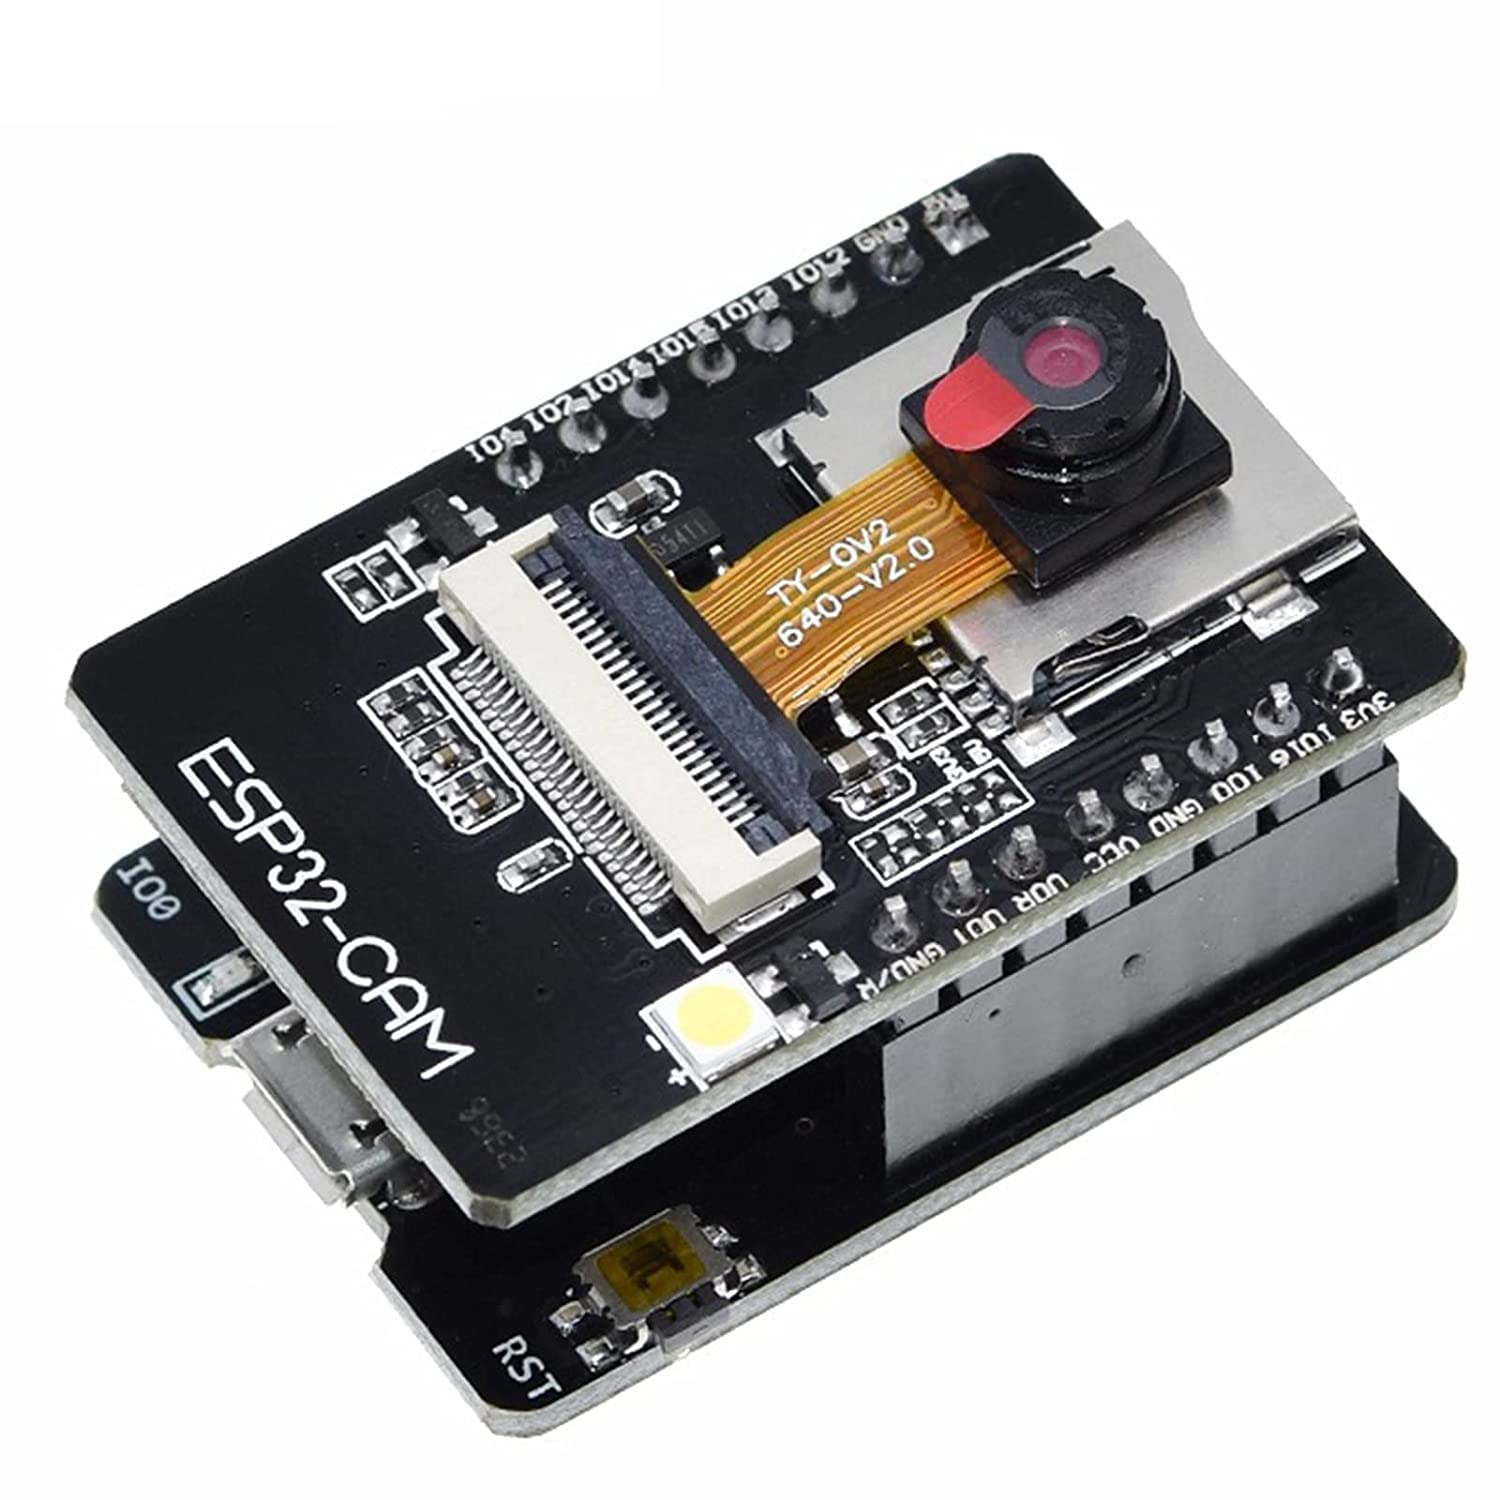
\includegraphics[width=0.3\textwidth]{imgs/Roboter/Real/esp32.jpg}
        \caption{ESP32 Microcontroller}
        \label{fig:esp32_mc}%
    \end{figure}

    Dieser muss natürlich auch mit Spannung versogt werden.
    Urprünglich waren sogenannte 18650 LiIon Akkus geplant. Allerdings wurde diese Idee verworfen da Sie doch mit viel Aufwand verbunden war.
    Inzwischen nutzen wir wiederaufladbare 9V Block Batterien. Die Akkus haben die perfekte Größe für unseren kleinen Roboter.

    Die Versorgungsspannung für die Motoren kann direkt von unserem Akkupack abgegriffen werden und zur H-Brücke geführt werden.
    Die H-Brücke benötigt genau so wie der ESP32 eine Versorgungsspannung für die Logik.
    Diese sollte laut Datenblatt bei 5V liegen, erlaubt sind aber auch 3V. Was in unserem Fall ideal ist da unser ESP32
    ebenfalls nur mit 3,3V maxmimal versorgt werden darf.

    Die 3,3V Logikspannung werden auf unserer Platine von einem LM317T, einem Lineareren Spannungswandler zur Verfügung gestellt.

    \begin{figure}[h!]
        \centering
        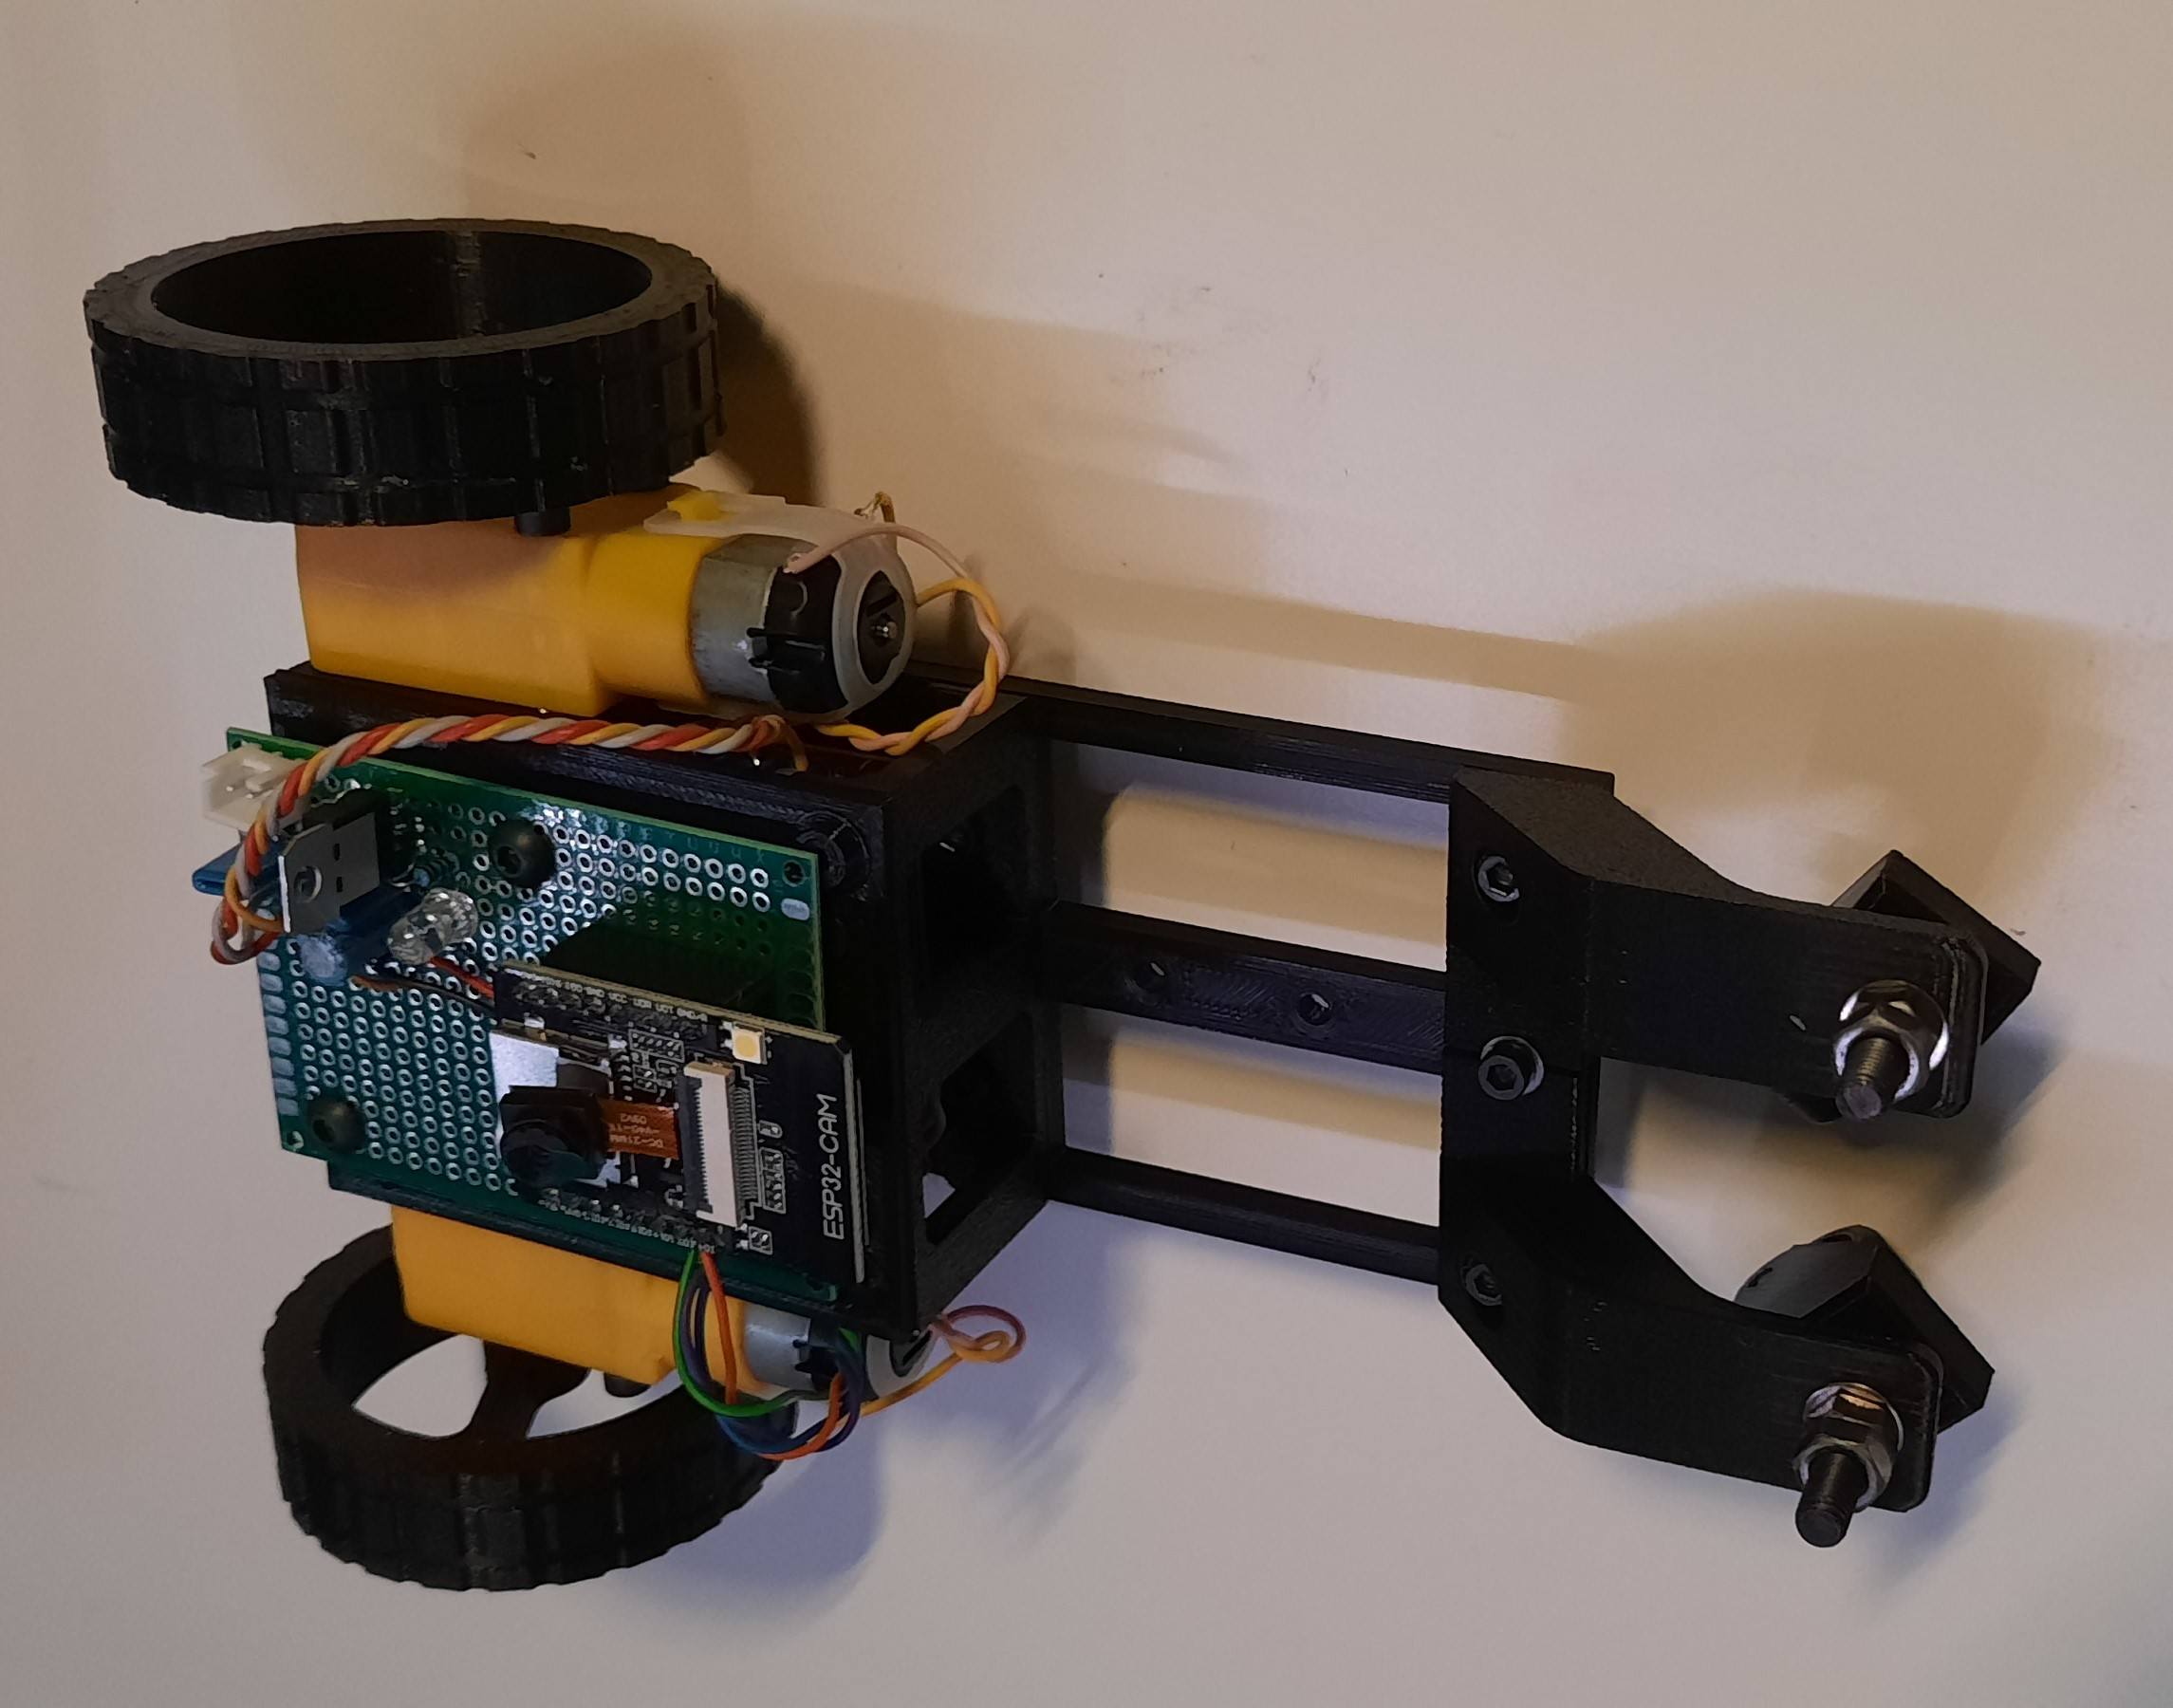
\includegraphics[width=0.4\textwidth, angle=180,origin=c]{imgs/Roboter/Real/Roboter.jpg}
        \caption{Roboter Demo Platform}
    \end{figure}

    Da durch die Verwendung der 9V Blockbatterie die Versorgungsspannung der Motoren nun die maximal zulässigen 6V
    überschreitet ist ein zweiter Spannungsregler von nöten der sich um die Reduzierung der Motorenspannung kümmert.
    Das ganze hat aber auch einen Vorteil da wir nun sehr große Freiheit haben was die Akkuspannung angeht. Theoretisch möglich wären nun bis zu 37V.

\end{flushleft}